\subsection{Seismic Inversion}

In this experiment we demonstrate the \eks and \uks performing a
one-dimensional seismic inversion. The goal is to infer the geometry of
different subsurface geological layers and the seismic propagation velocity
within each layer from noisy (interpreted) surface observations of sound
reflection times, \Outs. We use two datasets for this experiment; a simulated
world with two randomly generated splines representing geological layers (so we
have ground-truth), and a real seismic line from Otway basin (Pretty Hill
formation) which has four geological layers \fix{credit}. Each dataset has 50
and 113 observations per layer respectively.

The inputs, $\Ins$, are the surface locations (metres) of the seismic sensors,
and we use the following forward model,
\begin{align}
    \latents_p^\text{depth} &= \max\cbrac{\latents_p^\text{depth, input},
        \latents_{p-1}^\text{depth}} \quad \forall p, \label{eq:clip} \\
    \nonlinf_p^\text{time} &=
    \begin{cases}
        2\frac{\latents_p^\text{depth} - \latents_{p-1}^\text{depth}}
        {\latents_p^\text{vel}} + \nonlinf_{p-1}^\text{time},
        & \text{if } p > 0 \\
        2\frac{\latents_0^\text{depth}}{\latents_0^\text{vel}},
        & \text{if } p = 0
    \end{cases}
\end{align}
Where there are $\otdim$ output tasks -- reflection times from each layer,
$\nonlinf_p^\text{time}$, and there are two types of latent input tasks;
\begin{itemize}
    \item $\latents_p^\text{depth}\!\brac{\Ins}$, the geological depth of layer
        $p$ corresponding to each surface location. Equation \eqref{eq:clip} 
        clips overlapping estimated (input) layers to create these valid
        layers.
    \item $\latents_p^\text{vel}\!\brac{\Ins}$, the velocity of layer $p$ 
        corresponding to each surface location.
\end{itemize}
Each of these input tasks corresponds to an output task, so we have also
indexed by $p$ instead of $q$. Naturally then $\ltdim = 2\otdim$, and the
problem is under-constrained since there is an infinite set of layer depths and
velocities that can generate the reflection times. To help constrain our
models, we put a prior on the average depth of each layer.

We compare against two baseline methods, the first baseline model is a
(gradient free) maximum a-posteriori approach that optimises the latent task
points directly \fix{details below/supp material}. The second is a
probabilistic approach which parameterises the latent tasks as splines (to keep
dimensionality low) and learns the locations of the knot points using MCMC
\fix{cite stateline, see below/supp material for details.}

\begin{figure}
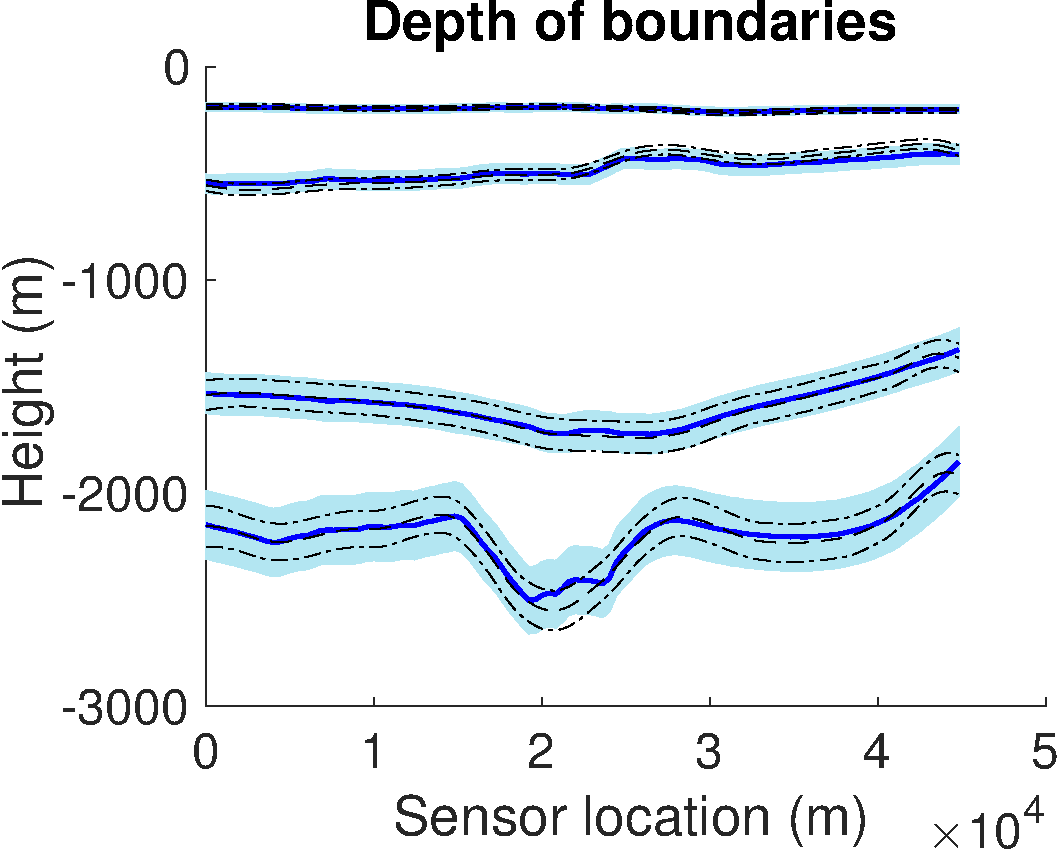
\includegraphics[width=0.4\textwidth]{seismicData-depth-Taylor-1000} \\
\includegraphics[width=0.4\textwidth]{seismicData-vel-Taylor-1000}
\caption{The inferred layer boundaries (top) seismic velocities on
 on the seismic inversion problem. }
\end{figure}

\fix{TODO}:
\begin{itemize}
    \item NLPD and MSE on the simulation data
    \item Plot of the Otway data
\end{itemize}
